% Created by tikzDevice version 0.10.1 on 2016-09-01 15:49:58
% !TEX encoding = UTF-8 Unicode
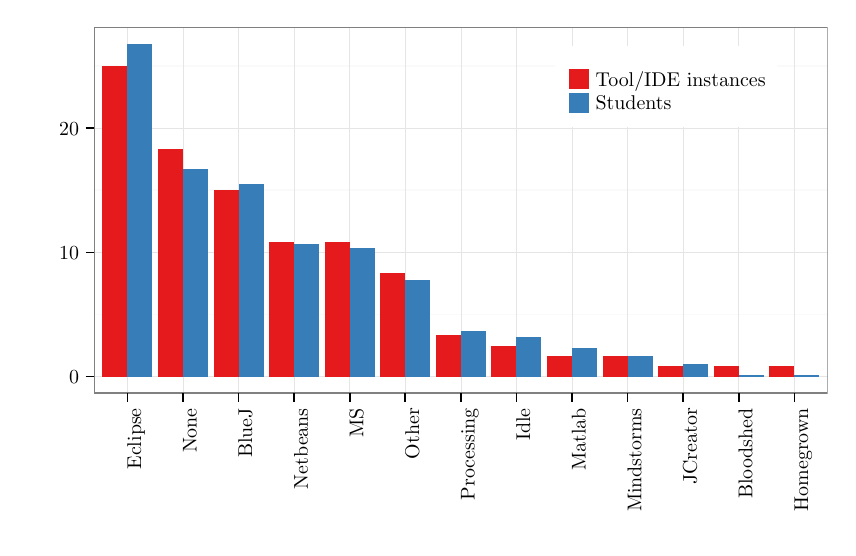
\begin{tikzpicture}[x=1pt,y=1pt]
\definecolor{fillColor}{RGB}{255,255,255}
\path[use as bounding box,fill=fillColor,fill opacity=0.00] (0,0) rectangle (289.08,180.67);
\begin{scope}
\path[clip] (  0.00,  0.00) rectangle (289.08,180.67);
\definecolor{drawColor}{RGB}{255,255,255}
\definecolor{fillColor}{RGB}{255,255,255}

\path[draw=drawColor,line width= 0.6pt,line join=round,line cap=round,fill=fillColor] (  0.00,  0.00) rectangle (289.08,180.68);
\end{scope}
\begin{scope}
\path[clip] ( 23.98, 48.58) rectangle (289.08,180.67);
\definecolor{fillColor}{RGB}{255,255,255}

\path[fill=fillColor] ( 23.98, 48.58) rectangle (289.08,180.67);
\definecolor{drawColor}{gray}{0.98}

\path[draw=drawColor,line width= 0.6pt,line join=round] ( 23.98, 77.03) --
	(289.08, 77.03);

\path[draw=drawColor,line width= 0.6pt,line join=round] ( 23.98,121.91) --
	(289.08,121.91);

\path[draw=drawColor,line width= 0.6pt,line join=round] ( 23.98,166.79) --
	(289.08,166.79);
\definecolor{drawColor}{gray}{0.90}

\path[draw=drawColor,line width= 0.2pt,line join=round] ( 23.98, 54.59) --
	(289.08, 54.59);

\path[draw=drawColor,line width= 0.2pt,line join=round] ( 23.98, 99.47) --
	(289.08, 99.47);

\path[draw=drawColor,line width= 0.2pt,line join=round] ( 23.98,144.35) --
	(289.08,144.35);

\path[draw=drawColor,line width= 0.2pt,line join=round] ( 36.03, 48.58) --
	( 36.03,180.67);

\path[draw=drawColor,line width= 0.2pt,line join=round] ( 56.11, 48.58) --
	( 56.11,180.67);

\path[draw=drawColor,line width= 0.2pt,line join=round] ( 76.20, 48.58) --
	( 76.20,180.67);

\path[draw=drawColor,line width= 0.2pt,line join=round] ( 96.28, 48.58) --
	( 96.28,180.67);

\path[draw=drawColor,line width= 0.2pt,line join=round] (116.36, 48.58) --
	(116.36,180.67);

\path[draw=drawColor,line width= 0.2pt,line join=round] (136.45, 48.58) --
	(136.45,180.67);

\path[draw=drawColor,line width= 0.2pt,line join=round] (156.53, 48.58) --
	(156.53,180.67);

\path[draw=drawColor,line width= 0.2pt,line join=round] (176.61, 48.58) --
	(176.61,180.67);

\path[draw=drawColor,line width= 0.2pt,line join=round] (196.70, 48.58) --
	(196.70,180.67);

\path[draw=drawColor,line width= 0.2pt,line join=round] (216.78, 48.58) --
	(216.78,180.67);

\path[draw=drawColor,line width= 0.2pt,line join=round] (236.86, 48.58) --
	(236.86,180.67);

\path[draw=drawColor,line width= 0.2pt,line join=round] (256.95, 48.58) --
	(256.95,180.67);

\path[draw=drawColor,line width= 0.2pt,line join=round] (277.03, 48.58) --
	(277.03,180.67);
\definecolor{fillColor}{RGB}{228,26,28}

\path[fill=fillColor] ( 26.99, 54.59) rectangle ( 36.03,166.79);
\definecolor{fillColor}{RGB}{55,126,184}

\path[fill=fillColor] ( 36.03, 54.59) rectangle ( 45.07,174.67);
\definecolor{fillColor}{RGB}{228,26,28}

\path[fill=fillColor] ( 47.08, 54.59) rectangle ( 56.11,136.87);
\definecolor{fillColor}{RGB}{55,126,184}

\path[fill=fillColor] ( 56.11, 54.59) rectangle ( 65.15,129.65);
\definecolor{fillColor}{RGB}{228,26,28}

\path[fill=fillColor] ( 67.16, 54.59) rectangle ( 76.20,121.91);
\definecolor{fillColor}{RGB}{55,126,184}

\path[fill=fillColor] ( 76.20, 54.59) rectangle ( 85.23,124.14);
\definecolor{fillColor}{RGB}{228,26,28}

\path[fill=fillColor] ( 87.24, 54.59) rectangle ( 96.28,103.21);
\definecolor{fillColor}{RGB}{55,126,184}

\path[fill=fillColor] ( 96.28, 54.59) rectangle (105.32,102.47);
\definecolor{fillColor}{RGB}{228,26,28}

\path[fill=fillColor] (107.33, 54.59) rectangle (116.36,103.21);
\definecolor{fillColor}{RGB}{55,126,184}

\path[fill=fillColor] (116.36, 54.59) rectangle (125.40,101.07);
\definecolor{fillColor}{RGB}{228,26,28}

\path[fill=fillColor] (127.41, 54.59) rectangle (136.45, 91.99);
\definecolor{fillColor}{RGB}{55,126,184}

\path[fill=fillColor] (136.45, 54.59) rectangle (145.48, 89.58);
\definecolor{fillColor}{RGB}{228,26,28}

\path[fill=fillColor] (147.49, 54.59) rectangle (156.53, 69.55);
\definecolor{fillColor}{RGB}{55,126,184}

\path[fill=fillColor] (156.53, 54.59) rectangle (165.57, 71.21);
\definecolor{fillColor}{RGB}{228,26,28}

\path[fill=fillColor] (167.58, 54.59) rectangle (176.61, 65.81);
\definecolor{fillColor}{RGB}{55,126,184}

\path[fill=fillColor] (176.61, 54.59) rectangle (185.65, 69.00);
\definecolor{fillColor}{RGB}{228,26,28}

\path[fill=fillColor] (187.66, 54.59) rectangle (196.70, 62.07);
\definecolor{fillColor}{RGB}{55,126,184}

\path[fill=fillColor] (196.70, 54.59) rectangle (205.73, 65.05);
\definecolor{fillColor}{RGB}{228,26,28}

\path[fill=fillColor] (207.74, 54.59) rectangle (216.78, 62.07);
\definecolor{fillColor}{RGB}{55,126,184}

\path[fill=fillColor] (216.78, 54.59) rectangle (225.82, 62.03);
\definecolor{fillColor}{RGB}{228,26,28}

\path[fill=fillColor] (227.83, 54.59) rectangle (236.86, 58.33);
\definecolor{fillColor}{RGB}{55,126,184}

\path[fill=fillColor] (236.86, 54.59) rectangle (245.90, 59.24);
\definecolor{fillColor}{RGB}{228,26,28}

\path[fill=fillColor] (247.91, 54.59) rectangle (256.95, 58.33);
\definecolor{fillColor}{RGB}{55,126,184}

\path[fill=fillColor] (256.95, 54.59) rectangle (265.98, 55.17);
\definecolor{fillColor}{RGB}{228,26,28}

\path[fill=fillColor] (267.99, 54.59) rectangle (277.03, 58.33);
\definecolor{fillColor}{RGB}{55,126,184}

\path[fill=fillColor] (277.03, 54.59) rectangle (286.07, 55.17);
\definecolor{drawColor}{gray}{0.50}

\path[draw=drawColor,line width= 0.6pt,line join=round,line cap=round] ( 23.98, 48.58) rectangle (289.08,180.67);
\end{scope}
\begin{scope}
\path[clip] (  0.00,  0.00) rectangle (289.08,180.67);
\definecolor{drawColor}{RGB}{0,0,0}

\node[text=drawColor,anchor=base east,inner sep=0pt, outer sep=0pt, scale=  0.72] at ( 18.58, 52.11) {0};

\node[text=drawColor,anchor=base east,inner sep=0pt, outer sep=0pt, scale=  0.72] at ( 18.58, 96.99) {10};

\node[text=drawColor,anchor=base east,inner sep=0pt, outer sep=0pt, scale=  0.72] at ( 18.58,141.87) {20};
\end{scope}
\begin{scope}
\path[clip] (  0.00,  0.00) rectangle (289.08,180.67);
\definecolor{drawColor}{RGB}{0,0,0}

\path[draw=drawColor,line width= 0.6pt,line join=round] ( 20.98, 54.59) --
	( 23.98, 54.59);

\path[draw=drawColor,line width= 0.6pt,line join=round] ( 20.98, 99.47) --
	( 23.98, 99.47);

\path[draw=drawColor,line width= 0.6pt,line join=round] ( 20.98,144.35) --
	( 23.98,144.35);
\end{scope}
\begin{scope}
\path[clip] (  0.00,  0.00) rectangle (289.08,180.67);
\definecolor{drawColor}{RGB}{0,0,0}

\path[draw=drawColor,line width= 0.6pt,line join=round] ( 36.03, 45.58) --
	( 36.03, 48.58);

\path[draw=drawColor,line width= 0.6pt,line join=round] ( 56.11, 45.58) --
	( 56.11, 48.58);

\path[draw=drawColor,line width= 0.6pt,line join=round] ( 76.20, 45.58) --
	( 76.20, 48.58);

\path[draw=drawColor,line width= 0.6pt,line join=round] ( 96.28, 45.58) --
	( 96.28, 48.58);

\path[draw=drawColor,line width= 0.6pt,line join=round] (116.36, 45.58) --
	(116.36, 48.58);

\path[draw=drawColor,line width= 0.6pt,line join=round] (136.45, 45.58) --
	(136.45, 48.58);

\path[draw=drawColor,line width= 0.6pt,line join=round] (156.53, 45.58) --
	(156.53, 48.58);

\path[draw=drawColor,line width= 0.6pt,line join=round] (176.61, 45.58) --
	(176.61, 48.58);

\path[draw=drawColor,line width= 0.6pt,line join=round] (196.70, 45.58) --
	(196.70, 48.58);

\path[draw=drawColor,line width= 0.6pt,line join=round] (216.78, 45.58) --
	(216.78, 48.58);

\path[draw=drawColor,line width= 0.6pt,line join=round] (236.86, 45.58) --
	(236.86, 48.58);

\path[draw=drawColor,line width= 0.6pt,line join=round] (256.95, 45.58) --
	(256.95, 48.58);

\path[draw=drawColor,line width= 0.6pt,line join=round] (277.03, 45.58) --
	(277.03, 48.58);
\end{scope}
\begin{scope}
\path[clip] (  0.00,  0.00) rectangle (289.08,180.67);
\definecolor{drawColor}{RGB}{0,0,0}

\node[text=drawColor,rotate= 90.00,anchor=base east,inner sep=0pt, outer sep=0pt, scale=  0.72] at ( 40.99, 43.18) {Eclipse};

\node[text=drawColor,rotate= 90.00,anchor=base east,inner sep=0pt, outer sep=0pt, scale=  0.72] at ( 61.07, 43.18) {None};

\node[text=drawColor,rotate= 90.00,anchor=base east,inner sep=0pt, outer sep=0pt, scale=  0.72] at ( 81.15, 43.18) {BlueJ};

\node[text=drawColor,rotate= 90.00,anchor=base east,inner sep=0pt, outer sep=0pt, scale=  0.72] at (101.24, 43.18) {Netbeans};

\node[text=drawColor,rotate= 90.00,anchor=base east,inner sep=0pt, outer sep=0pt, scale=  0.72] at (121.32, 43.18) {MS};

\node[text=drawColor,rotate= 90.00,anchor=base east,inner sep=0pt, outer sep=0pt, scale=  0.72] at (141.41, 43.18) {Other};

\node[text=drawColor,rotate= 90.00,anchor=base east,inner sep=0pt, outer sep=0pt, scale=  0.72] at (161.49, 43.18) {Processing};

\node[text=drawColor,rotate= 90.00,anchor=base east,inner sep=0pt, outer sep=0pt, scale=  0.72] at (181.57, 43.18) {Idle};

\node[text=drawColor,rotate= 90.00,anchor=base east,inner sep=0pt, outer sep=0pt, scale=  0.72] at (201.66, 43.18) {Matlab};

\node[text=drawColor,rotate= 90.00,anchor=base east,inner sep=0pt, outer sep=0pt, scale=  0.72] at (221.74, 43.18) {Mindstorms};

\node[text=drawColor,rotate= 90.00,anchor=base east,inner sep=0pt, outer sep=0pt, scale=  0.72] at (241.82, 43.18) {JCreator};

\node[text=drawColor,rotate= 90.00,anchor=base east,inner sep=0pt, outer sep=0pt, scale=  0.72] at (261.91, 43.18) {Bloodshed};

\node[text=drawColor,rotate= 90.00,anchor=base east,inner sep=0pt, outer sep=0pt, scale=  0.72] at (281.99, 43.18) {Homegrown};
\end{scope}
\begin{scope}
\path[clip] (  0.00,  0.00) rectangle (289.08,180.67);
\definecolor{fillColor}{RGB}{255,255,255}

\path[fill=fillColor] (190.59,144.93) rectangle (270.93,174.15);
\end{scope}
\begin{scope}
\path[clip] (  0.00,  0.00) rectangle (289.08,180.67);
\definecolor{fillColor}{RGB}{228,26,28}

\path[fill=fillColor] (195.57,158.44) rectangle (202.68,165.56);
\end{scope}
\begin{scope}
\path[clip] (  0.00,  0.00) rectangle (289.08,180.67);
\definecolor{fillColor}{RGB}{55,126,184}

\path[fill=fillColor] (195.57,149.91) rectangle (202.68,157.02);
\end{scope}
\begin{scope}
\path[clip] (  0.00,  0.00) rectangle (289.08,180.67);
\definecolor{drawColor}{RGB}{0,0,0}

\node[text=drawColor,anchor=base west,inner sep=0pt, outer sep=0pt, scale=  0.72] at (205.20,159.52) {Tool/IDE instances};
\end{scope}
\begin{scope}
\path[clip] (  0.00,  0.00) rectangle (289.08,180.67);
\definecolor{drawColor}{RGB}{0,0,0}

\node[text=drawColor,anchor=base west,inner sep=0pt, outer sep=0pt, scale=  0.72] at (205.20,150.99) {Students};
\end{scope}
\end{tikzpicture}
